\chapter{Conjuntos de números}

\section{El sistema de numeración decimal}

El sistema numérico que más solemos utilizar es el \textbf{sistema de numeración decimal} o simplemente \textbf{sistema decimal}. Éste es un sistema \textbf{posicional}. 

\subsection{¿Qué significa decimal?}

Pues que toma como base el número $10$, esto quiere decir que representamos las cantidades tomando como base aritmética el número diez y sus potencias (profundizaremos en las potencias más adelante). Para representar cualquier número tenemos disponibles diez dígitos: $\{0, 1, 2, 3, 4, 5, 6, 7, 8, 9\}$.

\begin{ejemplos}[label={Ejemplo:descomposicionPotencias10}]{Descomposición en potencias de 10}
    $5 = 5 \cdot 10^0$ \\
    $28 = 2 \cdot 10^1 + 8 \cdot 10^0$ \\
    $136 = 1 \cdot 10^2 + 3 \cdot 10^1 + 6 \cdot 10^0$ \\
    $\vdots$
\end{ejemplos}

Los órdenes de unidades cambian en el décimo elemento, si estamos en la unidades, cuando llegamos al $9$, pasamos a las decenas. Si estamos en las decenas, cuando llegamos al $90$, pasamos a las centenas, la novena centena es $900$, después tenemos las unidades de millar y así sucesivamente.

\subsection{¿Qué significa que es posicional?}

Significa que las cifras tienen un valor diferente dependiendo de en qué posición estén en el número. Si $n$ es una cifra cualquiera y está en la posición de las unidades vale $n \cdot 10^0 = n \cdot 1 = n$; si está en la posición de las decenas vale $n \cdot 10^1 = n \cdot 10 = n0$; si está en la posición de las centenas, su valor será $n \cdot 10^2 = n \cdot 100 = n00$ y así sucesivamente.

\begin{ejemplos}[label={Ejemplo:valorCifras}]{El valor de las cifras en un número}
    En el número $33333$, la cifra $3$ se repite cinco veces, sin embargo, cada una tiene un valor diferente:

    $33333 = 3 \cdot 10^4 + 3 \cdot 10^3 + 3 \cdot 10^ 2 + 3 \cdot 10^1 + 3 \cdot 10^0 = 30000 + 3000 + 300 + 30 + 3$

    Visto de otra forma:

    $33333 = 3 DM + 3 UM + 3 C + 3 D + 3 U = 30000 + 3000 + 300 + 30 + 3$
\end{ejemplos}

\subsection{¿Cómo comparamos números?}

Para \textbf{comparar dos números} podemos encontrarnos con las siguientes situaciones:

\begin{itemize}
    \item \textbf{Los dos números tienen diferente cantidad de cifras.} En este caso será mayor el número que tenga mayor cantidad de cifras.
    \item \textbf{Los dos números tienen la misma cantidad de cifras.} En este otro caso, lo que tenemos que hacer es ir comparando cifra por cifra \textbf{de mayor orden de unidades a menor orden de unidades} hasta encontrar que en un mismo orden de unidades tenemos una diferencia. El número mayor será el que tenga la primera cifra diferente mayor.
\end{itemize}

\begin{ejemplos}[label={Ejemplo:comparacionNumeros}]{Cómo comparar dos números}
    \begin{itemize}
        \item \textbf{Primer caso}. ¿Cuál es mayor, $2354$ ó $12001$?

        Como $12001$ tiene $5$ cifras y $2354$ tiene $4$, el número mayor es $12001$.

        \item \textbf{Segundo caso}. ¿Cuál es mayor, $12001$ ó $12011$?

        Ahora tenemos dos números con $5$ cifras, así que comparamos el orden de unidades mayor, que en este caso son las decenas de millar; como en ambos casos, tenemos una decena de millar, comparamos las unidades de millar que también coinciden, $2$ en ambos casos. Seguimos comparando las centenas, que es $0$ en los dos números, pero en las decenas encontramos una diferencia: el primer número tiene $0$ decenas y el segundo tiene $1$ decena, así que concluuimos que $12011$ es mayor que $12001$.
    \end{itemize}
\end{ejemplos}

\subsection{¿Qué símbolos utilizamos para comparar números?}

Utilizamos unos símbolos a los que llamamos \textbf{\textit{relacionales}}. Éstos son:

\begin{multicols}{3}
    $> \quad$ Mayor que \\
    $\geq \quad$ Mayor o igual que \\
    $< \quad$ Menor que \\
    $\leq \quad$ Menor o igual que \\
    $= \quad$ Igual a \\
    $\neq \quad$ Distinto a
\end{multicols}

\section{El conjunto de los números naturales}

\subsection{¿Qué son los números naturales}

Los números naturales son los que utilizamos para contar u ordenar y pertenecen al conjunto de números enteros positivos.

El conjunto de los números naturales se representa por $\mathbb{N}$ y está formado por $\mathbb{N} = \{ 0, 1, 2, 3, 4, 5,$ $\hdots \}$

Algunos autores piensan que el $0$ es un número natural y otros piensan que no lo es, pero nosotros, vamos a considerar que sí lo es.

Los números naturales no tienen decimal, unidad imaginaria, o bien no son fracciones.

Los números naturales son \textbf{ilimitados}, si a un número natural le sumamos $1$, obtenemos otro número natural.

\subsection{Cardinales y ordinales}

Si utilizamos los números naturales para contar, los llamamos \textbf{cardinales}, pero si los usamos para ordenar, los llamamos \textbf{ordinales}. Éstos últimos nos sirven para indicar orden o posición. Algunos números ordinales son:

\begin{center}
    \begin{multicols}{3}
        $1^{\circ} \rightarrow$ Primero \\
        $2^{\circ} \rightarrow$ Segundo \\
        $3^{\circ} \rightarrow$ Tercero \\
        $4^{\circ} \rightarrow$ Cuarto \\
        $5^{\circ} \rightarrow$ Quinto \\
        $6^{\circ} \rightarrow$ Sexto \\
        $7^{\circ} \rightarrow$ Séptimo \\
        $8^{\circ} \rightarrow$ Octavo \\
        $9^{\circ} \rightarrow$ Noveno \\
        $10^{\circ} \rightarrow$ Décimo \\
        $11^{\circ} \rightarrow$ Undécimo \\
        $12^{\circ} \rightarrow$ Duodécimo \\
        $13^{\circ} \rightarrow$ Decimotercero \\
        $20^{\circ} \rightarrow$ Vigésimo \\
        $21^{\circ} \rightarrow$ Vigésimo primero \\
        $22^{\circ} \rightarrow$ Vigésimo segundo \\
        $30^{\circ} \rightarrow$ Trigésimo \\
        $40^{\circ} \rightarrow$ Cuadragésimo \\
        $50^{\circ} \rightarrow$ Quincuagésimo \\
        $60^{\circ} \rightarrow$ Sexagésimo \\
        $70^{\circ} \rightarrow$ Septuagésimo \\
        $80^{\circ} \rightarrow$ Octogésimo \\
        $90^{\circ} \rightarrow$ Nonagésimo \\
        $100^{\circ} \rightarrow$ Centésimo
    \end{multicols}
\end{center}

\subsection{Redondeo}

Redondear es aproximar un número a un determinado orden de unidades. Para redondear un número a un determinado orden de unidades, se sustituyen por ceros las cifras a la derecha de ese orden de unidades. Si la primera cifra sustituida es 5 o mayor que 5, se suma 1 a la cifra anterior.

\begin{ejemplos}[label={Ejemplo:redondeo}]{Redondeo de números}
    \begin{itemize}
        \item Queremos redondear 53356678 a las decenas de millón $\rightarrow 50000000$
        \item Queremos redondear 53356678 a las unidades de millar $\rightarrow 53357000$
    \end{itemize}
\end{ejemplos}

\subsection{Propiedades}

\subsubsection{Propiedad conmutativa de la suma}

En una suma podemos ordenar los \textbf{sumandos} como queramos porque el resultado o \textbf{suma} no cambiará.

\begin{ejemplos}[label={Ejemplo:conmutativa}]{Propiedad conmutativa de la suma}
    \[3 + 2 = 2 + 3 = 5 \nonumber \]
\end{ejemplos}

\subsubsection{Relación entre la suma y la resta}

En una resta tenemos tres términos: \textbf{minuendo}, \textbf{sustraendo} y \textbf{diferencia}.

\begin{center}
    \begin{tabular}{ccc}
         & 5 & $\rightarrow$ Minuendo\\
        - & 2 & $\rightarrow$ Sustraendo\\
        \hline
        & 3 & $\rightarrow$ Diferencia
    \end{tabular}
\end{center}

Si sumamos el sustraendo y la diferencia, obtendremos el minuendo:

\[M = S + D \nonumber \]

Si conocemos dos de los términos de la resta, podemos conocer el valor del término que nos falta aislándolo en la ecuación anterior:

\[D = M - S \nonumber \]
\[S = M - D \nonumber \]

\begin{ejemplos}[label={Ejemplo:relacionsumaresta}]{Relación entre la suma y la resta}
    \begin{center}
        \begin{tabular}{ccc}
            \opsub{5}{2} & \opadd{2}{3} & \opsub{5}{3} \\
            $D = M - S$ \qquad &$ M = S + D$ \qquad & $S = M - D$ \qquad
        \end{tabular}
    \end{center}
\end{ejemplos}

\subsubsection{Propiedad asociativa de la suma}

Si queremos sumar tres o más números podemos agruparlos como queramos que el resultado o suma no cambiará.

\begin{ejemplos}[label={Ejemplo:asociativa}]{Propiedad asociativa de la suma}
    \[3 + 5 + 7 = (3 + 5) + 7 = 3 + (5 + 7) = 15 \nonumber \]
\end{ejemplos}

\subsubsection{Propiedad distributiva de la suma o de la resta respecto del producto}

Si multiplicamos el resultado de una suma (o resta) por un número, obtenemos el mismo resultado que si multiplicamos cada término de la suma (o resta) por ese número y luego los sumamos o los restamos.

\begin{ejemplos}[label={Ejemplo:distributiva}]{Propiedad distributiva respecto de la suma y de la resta}
    \begin{gather*}
        (5 + 2) \cdot 3 = 3 \cdot 5 + 3 \cdot 2 = 21 \\
        (5 + 2) \cdot 3 = 7 \cdot 3 = 21 \\
        3 \cdot 5 + 3 \cdot 2 = 15 + 6 = 21
    \end{gather*}

    \begin{gather*}
        (5 - 2) \cdot 3 = 3 \cdot 5 - 3 \cdot 2 = 9 \\
        (5 - 2) \cdot 3 = 3 \cdot 3 = 9 \\
        3 \cdot 5 - 3 \cdot 2 = 15 - 6 = 9
    \end{gather*}
\end{ejemplos}

\vspace{3mm}
Cuando hay varias sumas, restas o sumas y restas con un término común, se pueden convertir esas sumas y restas en un producto. Es el proceso inverso de la propiedad distributiva y lo llamamos \textbf{sacar factor común}.

\begin{ejemplos}[label={Ejemplo:factorcomun}]{Sacar factor común}
    \begin{gather*}
        5 \cdot 2 + 7 \cdot 2 - 3 \cdot 2 = 2 \cdot (5 + 7 - 3) = 18 \\
        5 \cdot 2 + 7 \cdot 2 - 3 \cdot 2 = 10 + 14 - 6 = 18 \\
        2 \cdot (5 + 7 - 3) = 2 \cdot 9 = 18
    \end{gather*}
\end{ejemplos}

\subsection{Operaciones combinadas}

En ocasiones nos encontraremos con operaciones diferentes en la misma expresión. Cuando esto sucede, tenemos que tener muy claro cuál será el orden en el que iremos resolviendo dichas operaciones para que el resultado sea correcto. Ese orden es el siguiente:

\begin{enumerate}
    \item Resolvemos las operaciones que están entre paréntesis.
    \item Resolvemos los productos y las divisiones.
    \item Resolvemos las sumas y las restas.
    \item En el caso en el que haya varias operaciones del mismo orden (por ejemplo, varias sumas y restas seguidas), resolveremos de izquierda a derecha.
\end{enumerate}

\begin{ejemplos}[label={Ejemplo:operacionescombinadas}]{Operaciones combinadas}
    \begin{gather*}
        38 - 72 : 24 + 7 - (2 - 1) \\
        38 - 72 : 24 + 7 - 1 \\
        38 - 3 + 7 - 1 \\
        35 + 7 - 1 \\
        42 - 1 \\
        41
    \end{gather*}
\end{ejemplos}

\section{Números enteros}

\subsection{¿Qué son los números enteros?}

El conjunto de los números enteros está formado por los números naturales, sus opuestos (negativos) y el cero. Lo representamos con $\mathbb{Z}$ y está formado por $\mathbb{Z} = \{ \hdots, -3, -2, -1, 0, 1, 2, 3,$ $\hdots \}$

Los número enteros se dividen en tres partes:

\begin{itemize}
    \item Enteros positivos o naturales.
    \item Enteros negativos.
    \item Cero.
\end{itemize}

Dado que los enteros contienen los enteros positivos, se considera a los números naturales como un subconjunto de los enteros, esto es, \textbf{los números enteros contienen a los números naturales}.

\subsubsection{¿Para qué sirven los números enteros?}

Se pueden utilizar, entre muchas otras cosas, para representar el dinero que se debe, la profundidad con respecto al nivel del mar, las temperaturas sobre y bajo cero o las plantas de un edificio (por encima y por debajo del nivel de la calle).

\subsection{¿Cómo sumamos los números enteros?}

Cuando sumamos números enteros, podemos encontrarnos con dos situaciones:

\begin{itemize}
    \item \textbf{Los números que sumamos tienen el mismo signo:}
    \begin{itemize}
        \item Primero nos olvidamos del signo y \textbf{sumamos} los números.
        \item Después ponemos al resultado el signo que tenían los números que estábamos sumando.
        \begin{ejemplos}[label={Ejemplo:sumaEnterosMismoSigno}]{Suma de enteros con el mismo signo}
            \begin{gather}
                +2 + (+5) = +7 \nonumber \\
                -2 + (-5) = -7 \nonumber
            \end{gather}
        \end{ejemplos}
    \end{itemize}
    \item \textbf{Los números que sumamos tienen diferente signo:}
    \begin{itemize}
        \item Primero nos olvidamos del signo y \textbf{restamos} el número menor al número mayor.
        \item Después ponemos al resultado el signo que tenía el mayor de los números con los que estábamos operando.
        \begin{ejemplos}[label={Ejemplo:sumaEnterosDistintoSigno}]{Suma de enteros con distinto signo}
            \begin{gather}
                -2 + (+5) = +3 \nonumber \\
                +2 + (-5) = -3 \nonumber
            \end{gather}
        \end{ejemplos}
    \end{itemize}
\end{itemize}

Cuando decimos que ``nos olvidamos del signo'', lo que estamos haciendo es trabajar con el \textbf{valor absoluto} del número. El valor absoluto de un número es su valor sin tener en cuenta su signo.

\begin{ejemplos}[label={Ejemplo:valorAbsoluto}]{Valor absoluto}
    \begin{itemize}
        \item El \textbf{valor absoluto} de $+4$ es $4$.
        \item El \textbf{valor absoluto} de $-4$ es $4$.
    \end{itemize}
\end{ejemplos}

\subsection{¿Cómo ordenamos los números enteros?}

Al comparar números enteros tendremos en cuenta lo siguiente:

\begin{enumerate}
    \item Cualquier número positivo es mayor que cualquier número negativo.
    \[+8 > -5\]
    \[+5 > -7\]
    \item Cualquier número situado a la derecha de otro en la recta numérica es mayor que este.
    \[-2 > -5\]
\end{enumerate}

\begin{center}
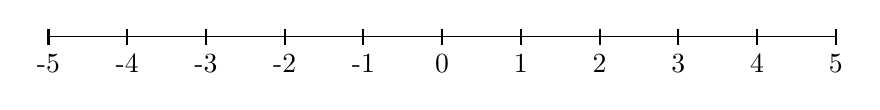
\begin{tikzpicture}
\draw (-5,0) -- (5,0);
\foreach \x in {-5,...,5}
\draw[line width = 0.8] (\x,0.1) -- (\x,-0.1) node[below]{\x};
\end{tikzpicture}
\end{center}

\subsection{¿Qué es el plano cartesiano?}

Si nos fijamos en un plano cartesiano, podemos ver que tiene números negativos (izquierda y abajo de centro) y números positivos (derecha y arriba del centro).

El plano cartesiano son dos rectas perpendiculares que se cortan en un punto que se denomina \textbf{origen de coordenadas}.

\begin{itemize}
    \item Las rectas dividen el plano en cuatro cuadrantes: primer cuadrante situado arriba a la derecha (positivo, positivo); segundo cuadrante situado arriba a la izquierda (negativo, positivo); tercer cuadrante situado abajo a la izquierda (negativo, negativo); cuarto cuadrante situado abajo a la derecha (positivo, negativo).
    \item La localización de cada punto del plano se identifica por sus coordenadas. Primero se lee la del eje horizontal y después la del eje vertical.
    \item Las coordenadas del origen son $(0, 0)$.
\end{itemize}

En la imagen siguiente se puede ver representado un punto de cada cuadrante y sus coordenadas:

\begin{figure}[!ht]
    \begin{center}
    \begin{tikzpicture}
        %Eje x
        \draw[->](-5, 0) -- (5, 0) node[below]{$x$};
        \foreach \x in {-4,...,-1,1,2,...,4} \draw[shift={(\x, 0)}] (0pt, 2pt) -- (0pt, -2pt) node[below]{\footnotesize $\x$};

        %Eje y
        \draw[->](0, -5) -- (0, 5) node[left]{$y$};
        \foreach \y in {-4,...,-1,1,2,...,4} \draw[shift={(0, \y)}] (-2pt, 0pt) -- (2pt, 0pt) node[left]{\footnotesize $\y$};

        %El origen
        \node[above left] at (0, 0) {\footnotesize $(0,0)$};

        %Con tkz-euclide
        %Define puntos
        \tkzDefPoint(0, 0){O}
        \tkzDefPoint(3, 2){A}
        \tkzDefPoint(-3, 2){B}
        \tkzDefPoint(-3, -2){C}
        \tkzDefPoint(1, -4){D}

        %Dibuja puntos
        \tkzDrawPoints(O, A, B, C, D)

        %Etiquetas de los puntos
        %\tkzLabelPoints[above](A)
        %\tkzLabelPoints[above](B)
        %\tkzLabelPoints[above](C)
        %\tkzLabelPoints[above](D)
        \node[above right] at (3, 2) {\footnotesize $A = (3, 2)$};
        \node[above left] at (-3, 2) {\footnotesize $B = (-3, 2)$};
        \node[below left] at (-3, -2) {\footnotesize $C = (-3, -2)$};
        \node[below right] at (1, -4) {\footnotesize $D = (1, -4)$};
    \end{tikzpicture}
    \end{center}
    \caption{Eje de coordenadas}
    \label{fig:eje-coordenadas}
\end{figure}

\section{Números racionales}

El conjunto de los números raciones es aquel en el que sus elementos se pueden representar como el cociente de dos números enteros, con denominador distinto de cero. Pueden tener forma de fracción: $\displaystyle \frac{1}{2}$ o forma de número decimal: $0.5$.

El conjunto de números enteros es un subconjunto del conjunto de los números racionales, o lo que es lo mismo, \textbf{el conjunto de números racionales contiene al conjunto de los números enteros}. Podemos escribir los números enteros como fracción:

\begin{ejemplos}[label={Ejemplo:enteroComoFraccion}]{Números enteros en forma de fracción}
    \begin{multicols}{2}
        \begin{center}
            $\displaystyle 5 = \frac{5}{1}$ \\
            $\displaystyle -7 = \frac{-7}{1}$
        \end{center}
    \end{multicols}
\end{ejemplos}

Una fracción es la expresión de las partes iguales que se toman de una unidad. El \textbf{denominador} indica las partes iguales en que se divide la unidad y el \textbf{numerador} las partes que se toman:

\begin{figure}[!ht]
    \begin{center}
    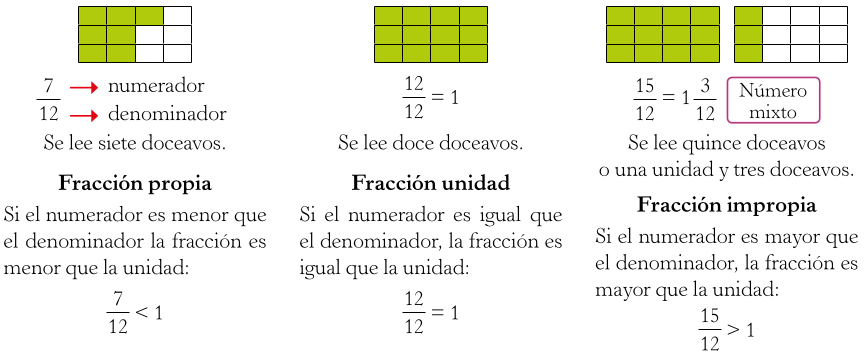
\includegraphics[scale=0.5]{imagenes/01_Tema01/fracciones01.png}
    \caption{Las fracciones}
    \label{fig:fracciones01}
    \end{center}
\end{figure}

\subsection{¿Cómo calculamos la fracción de una cantidad?}

Podemos calcular la fracción de una cantidad dividiendo la cantidad entre el denominador de la fracción y multiplicando el resultado por el numerador de la fracción. También lo podemos hacer al revés, multiplicando primero la cantidad por el numerador de la fracción y después dividiendo el resultado entre el denominador de la fracción.

\begin{ejemplos}[label={Ejemplo:fraccionCantidad}]{Cómo calcular la fracción de una cantidad}
    Calculamos $\displaystyle \frac{5}{8}$ de $32$:

    \begin{itemize}
        \item Dividimos $32$ entre el denominador, $8$, en este caso: \opdiv[style=text]{32}{8}.
        \item Multiplicamos el resultado anterior, $4$, por el numerador, $5$, en este ejemplo: \opmul[style=text]{4}{5}.
    \end{itemize}
    Así que tenemos que $\displaystyle \frac{5}{8}$ de $32 = 20$. Podéis comprobar que si cambiamos el orden de las operaciones, el resultado no varía.
\end{ejemplos}

\subsection{¿Cómo comparamos dos fracciones?}

Podemos encontrarnos con tres casos diferentes:

\begin{itemize}
    \item Las dos fracciones que quiero comparar tienen el \textbf{mismo denominador}. En este caso será mayor la que tenga mayor numerador.

    \begin{ejemplos}[label={Ejemplo:mismoDenominador}]{Comparo fracciones con el mismo denominador}
        \begin{center}
            $\displaystyle \frac{2}{3} < \frac{7}{3}$ \qquad ó \qquad $\displaystyle \frac{7}{3} > \frac{2}{3}$
        \end{center}
    \end{ejemplos}
    
    \item Las dos fracciones que quiero comparar tienen el \textbf{mismo numerador}. Este es el caso en el que la fracción mayor será la que tenga menor denominador.

    \begin{ejemplos}[label={Ejemplo:mismoNumerador}]{Comparo fracciones con el mismo numerador}
        \begin{center}
            $\displaystyle \frac{2}{3} > \frac{2}{5}$ \qquad ó \qquad $\displaystyle \frac{2}{5} < \frac{2}{3}$
        \end{center}
    \end{ejemplos}

    \item Las fracciones que quiero comparar tienen \textbf{distinto numerador y distinto denominador}. En este caso, tendremos que expresar las fracciones como decimales, es decir, tenemos que hacer la división y comparar los números decimales que corresponden a cada fracción.

    Otra forma de hacerlo es \textbf{reduciendo ambas fracciones a común denominador}, pero este método lo veremos en las próximas secciones.

    \begin{ejemplos}[label={Ejemplo:distintoNumeradorDenominador}]{Comparo fracciones con distinto numerador y distinto denominador}
        \begin{center}
            $\displaystyle \frac{3}{4} = 0.75 < \frac{4}{5} = 0.8$ \qquad ó \qquad $\displaystyle \frac{4}{5} > \frac{3}{4}$
        \end{center}
    \end{ejemplos}
\end{itemize}

Hay algunos casos en los que numerador y denominador son diferentes y no tenemos que hacer la división, por ejemplo, cuando una de las fracciones tiene el numerador mayor que el denominador y la otra tiene el numerador menor que el denominador; la que es más grande que la unidad (la primera) será mayor que la que es más pequeña que la unidad (la segunda).

\begin{ejemplos}[label={Ejemplo:mayorMenorUnidad}]{Comparo fracciones con distinto numerador y distinto denominador pero una mayor que la unidad y otra menor}
    \begin{center}
        $\displaystyle \left( \frac{3}{2} > 1 \right) > \left( \frac{4}{5} < 1 \right) $
    \end{center}
\end{ejemplos}

\subsection{¿Qué son las fracciones equivalentes?}

Dos o más fracciones son equivalentes cuando representan la misma cantidad. Cuando dos o más fracciones son equivalentes, los productos cruzados de sus términos son iguales:

\begin{center}
    $\displaystyle \frac{a}{b} = \frac{c}{d}$ \quad si \quad $a \cdot d = b \cdot c$
\end{center}

A partir de una fracción, podemos obtener fracciones equivalente por ampliación y por reducción (por reducción no siempre es posible):

\begin{itemize}
    \item \textbf{Fracciones equivalentes por ampliación}. Se obtienen multiplicando numerador y denominador por un mismo número cualquiera.

    \begin{ejemplos}[label={Ejemplo:ampliacion}]{Fracción equivalente por ampliación}
        \begin{center}
            $\displaystyle \frac{1}{2} = \frac{1 \cdot 3}{2 \cdot 3} = \frac{3}{6}$
        \end{center}
    \end{ejemplos}

    \item \textbf{Fracciones equivalentes por reducción o simplificación}. Se obtienen dividiendo numerador y denominador por un mismo número, aunque como hemos dicho antes, esto no siempre es posible.

    \begin{ejemplos}[label={Ejemplo:reduccion}]{Fracción equivalente por reducción (simplificación)}
        \begin{center}
            $\displaystyle \frac{4}{8} = \frac{4 \div 4}{8 \div 4} = \frac{1}{2}$
        \end{center}
    \end{ejemplos}

    \item Si una fracción no se puede simplificar porque no hay ningún número por el que podamos dividir numerador y denominador (esta división tiene que ser exacta), estaremos ante una \textbf{fracción irreducible}.

    \begin{ejemplos}[label={Ejemplo:irreducible}]{Fracciones irreducibles}
        \begin{center}
            $\displaystyle \frac{1}{2} \qquad \frac{2}{3} \qquad \frac{3}{2} \qquad \frac{4}{5}$
        \end{center}
    \end{ejemplos}
\end{itemize}

\subsubsection{¿Cómo calculamos la fracción irreducible de una fracción?}

\begin{itemize}
    \item Calculamos el máximo común divisor (m.c.d.).
    \item Dividimos numerador y denominador por el m.c.d.
\end{itemize}

\begin{ejemplos}[label={Ejemplo:mcd}]{Calculamos la fracción irreducible de una fracción}
    Tenemos la fracción $\displaystyle \frac{6}{12}$ y queremos calcular una equivalente irreducible si es que la hay:
    
    \begin{itemize}
        \item Calculo el m.c.d. de $6$ y $12$, por ejemplo así:

        \begin{itemize}
            \item Descompongo $6$ y $12$ en sus factores primos:

            \begin{center}
            \begin{tabular}{c|c}
                6 & 2 \\
                3 & 3 \\
                1
            \end{tabular} $\Rightarrow 6 = 2 \cdot 3$ \qquad
            \begin{tabular}{c|c}
                12 & 2 \\
                \phantom{a} 6 & 2 \\
                \phantom{a}  3 & 3 \\
                 \phantom{a} 1
            \end{tabular} $\Rightarrow 12 = 2^2 \cdot 3$
            \end{center}

            \item El m.c.d. son los factores comunes de $6$ y $12$ elevados al mínimo exponente:

            \begin{center}
                m.c.d. $= 2 \cdot 3 = 6$
            \end{center}
            
        \end{itemize}

        \item Divido el numerador y el denominador de $\displaystyle \frac{6}{12}$ entre $6$:

        \begin{center}
            $\displaystyle \frac{6 \div 6}{12 \div 6} = \frac{1}{2}$
        \end{center}
    \end{itemize}

    $\displaystyle \frac{1}{2}$ es la fracción irreducible de $\displaystyle \frac{6}{12}$.
\end{ejemplos}

\subsection{¿Cómo reducimos varias fracciones a común denominador?}

Reducir fracciones a común denominador es sustituirlas por otras equivalentes que tengan el mismo denominador. Para ello, seguimos los pasos siguientes:

\begin{itemize}
    \item Buscamos el mínimo común múltiplo (m.c.m.) de los denominadores.
    \item Sustituimos cada fracción por otra equivalente que tenga como denominador el m.c.m. de los denominadores y como numerador el resultado de dividir el m.c.m. entre el denominador original y multiplicarlo por el numerador original.
\end{itemize}

Veamos un ejemplo, vamos a reducir a común denominador las fracciones $\displaystyle \frac{3}{4}$ y $\displaystyle \frac{4}{5}$:

\begin{ejemplos}[label={Ejemplo:mcm}]{Calculamos el m.c.m.}
    Tenemos dos fracciones con distinto denominador: $\displaystyle \frac{3}{4}$ y $\displaystyle \frac{4}{5}$.

    \begin{itemize}
        \item Descomponemos los denominadores en factores primos:

        \begin{center}
            \begin{tabular}{c|c}
                4 & 2 \\
                2 & 2 \\
                1
            \end{tabular} $\Rightarrow 4 = 2^2$ \qquad
            \begin{tabular}{c|c}
                5 & 5 \\
                1 
            \end{tabular} $\Rightarrow 5 = 5$
        \end{center}

        \item El m.c.m. es el producto de los factores comunes y no comunes elevados al máximo exponente:

        m.c.m.(4, 5) $= 2^2 \cdot 5 = 20$

        \item Calculamos la fracción equivalente a $\displaystyle \frac{3}{4}$ dividiendo el m.c.m.(4, 5) entre $4$ y multiplicando el resultado por $3$:

        \begin{center}
            $\displaystyle 20 \div 4 = 5; \quad 5 \cdot3 = 15 \Rightarrow \frac{3}{4} = \frac{15}{20}$
        \end{center}

        \item Calculamos la fracción equivalente a $\displaystyle \frac{4}{5}$ dividiendo el m.c.m.(4, 5) entre $5$ y multiplicando el resultado por $4$:

        \begin{center}
            $\displaystyle 20 \div 5 = 4; \quad 4 \cdot 4 = 16 \Rightarrow \frac{4}{5} = \frac{16}{20}$
        \end{center}
    \end{itemize}

    Una vez reducidas ambas fracciones a común denominador tenemos dos fracciones equivalentes a las originales con el mismo denominador, esto nos permitirá compararlas o sumarlas entre otras operaciones.
\end{ejemplos}


\subsection{Suma y resta de fracciones}

Cuando queremos sumar o restar fracciones podemos encontrarnos con dos situaciones:

\begin{enumerate}
    \item \textbf{Las dos fracciones tienen el mismo denominador.}

    En este caso, el resultado será una fracción con el mismo denominador que los términos con los que tenemos quie operar y como numerador tendrá la suma o resta de los numeradores de las fracciones originales.

    \begin{ejemplos}[label={Ejemplo:sumaRestaFraccionesIgualDenominador}]{Suma y resta de fracciones con el mismo denominador}
        \begin{center}
            $\displaystyle \frac{2}{3} + \frac{4}{3} = \frac{6}{3} = 2$ \qquad \qquad $\displaystyle \frac{4}{3} - \frac{2}{3} = \frac{2}{3}$
        \end{center}
    \end{ejemplos}

    \item \textbf{Las fracciones tienen distinto denominador}.
    En este otro caso, primero tendremos que hallar fracciones equivalentes a las originales reduciendo a común denominador y luego sumar o restar como en el caso anterior.

    \begin{ejemplos}[label={sumaRestaFraccionesDistintoDenominador}]{Suma y resta de fracciones con distinto denominador}
        \begin{center}
            $\displaystyle \frac{3}{4} + \frac{4}{5} = \frac{15}{20} + \frac{16}{20} = \frac{31}{20}$ \qquad \qquad $\displaystyle \frac{4}{5} - \frac{3}{4} = \frac{16}{20} - \frac{15}{20} = \frac{1}{20}$
        \end{center}
        
    \end{ejemplos}
\end{enumerate}



\section{Números reales}